\section{Các khái niệm cần biết}
\subsection{Xử lý ảnh}
\subsubsection{Giới thiệu chung}
Xử lý ảnh là quá trình sử dụng máy tính để thu thập và phân tích các hình ảnh nhằm mục đích trích xuất, cải thiện hoặc biến đổi thông tin hình ảnh. Cụ thể, xử lý ảnh bao gồm các bước: thu thập ảnh, tiền xử lý (c ải thiện chất lượng), phân tích và nhận dạng (phân đoạn ảnh, chiết xuất đặc trưng), ra quyết định/dự đoán dựa trên kết quả phân tích.\\
\newline
Mục đích chính của xử lý ảnh là nâng cao chất lượng hình ảnh, nhận dạng các đối tượng (vật thể, khuôn mặt, chữ viết, v.v.) trong ảnh và hỗ trợ ra quyết định trong các hệ thống thông minh. Xử lý ảnh được ứng dụng rộng rãi trong y tế (phân tích Xquang, CT scanner), bảo mật (nhận dạng khuôn mặt), giao thông (nhận dạng biển báo, xe cộ), nông nghiệp (đánh giá chất lượng nông sản), v.v.
\subsubsection{Tensor trong xử lý ảnh}
Tensor là một khái niệm toán học dùng để biểu diễn dữ liệu đa chiều trong xử lý ảnh và thị giác máy tính.
\begin{itemize}
\item Vector 1D (tensor 1 chiều)
\item Ma trận 2D (tensor 2 chiều)
\item Tensor RGB 3D - [Chiều ảnh, Chiều cao, 3 kênh màu]
\end{itemize}
\newline
So với vector và ma trận thông thường, tensor có thể lưu trữ dữ liệu ở nhiều chiều, thể hiện cấu trúc dữ liệu phức tạp hơn.
Ví dụ:
%
%
%
%
\subsubsection{Convolution trong xử lý ảnh}
Convolution là một phép toán được sử dụng rộng rãi trong xử lý ảnh để tăng cường các đặc trưng mong muốn của ảnh.
\myparagraph{Định nghĩa Convolution}
Convolution là phép nhân 2 hàm f và g để tạo ra hàm mới h:

$h(t) = (f * g)(t) = \int_{-\infty}^{+\infty} f(\tau) g(t - \tau) d\tau$
\newline
Trong đó, $f$ là ảnh input, $g$ là bộ lọc (kernel) và $h$ là ảnh output.
Với mỗi phần tử xij trong ma trận X lấy ra một ma trận có kích thước bằng kích thước của kernel W có phần tử xij làm trung tâm (đây là vì sao kích thước của kernel thường lẻ) gọi là ma trận A. Sau đó tính tổng các phần tử của phép tính \textit{element-wise} của ma trận A và ma trận W, rồi viết vào ma trận kết quả Y.
\begin{equation}
    X=\begin{bmatrix}
        1 & 1 & 1 & 0 & 0 \\
        0 & \colorbox{yellow}{$1$} & 1 & 1 & 0 \\
        0 &  0 & 1 & 1 & 1\\
        0 & 0 & 1 & 1 & 0 \\
        0 & 1 & 1 & 0 & 0
    \end{bmatrix}
    \cdot
    W=\begin{bmatrix}
        1 & 0 & 1 \\
        0 & 1 & 0 \\
        1 & 0 & 1 
       
    \end{bmatrix}
    =
    Y=\begin{bmatrix}
        y_{11} & y_{12}& y_{13} \\
        y_{21} & y_{22}& y_{23} \\
        y_{31} & y_{32}& y_{33}\\
    \end{bmatrix}
\end{equation}
Ví dụ khi tính tại $x_{22}$, ma trận A cùng kích thước với W. Sau đó tính\[
y_{11} = x_{11} \cdot w_{11} + x_{12} \cdot w_{12} + x_{13} \cdot w_{13} + x_{21} \cdot w_{21} + x_{22} \cdot w_{22} + x_{23} \cdot w_{23} + x_{31} \cdot w_{31} + x_{32} \cdot w_{32} + x_{33} \cdot w_{33} = 4
\]

\myparagraph{Convolution trong xử lý ảnh}
Trong xử lý ảnh, convolution được dùng để:

\begin{itemize}
\item Làm nổi bật cạnh của các vật thể
\item Phát hiện các đặc trưng như cạnh, góc, đường thẳng, v.v.
\item Nhận dạng vật thể, khuôn mặt, chữ số, v.v.
\end{itemize}

\subsection{Padding và stride trong Convolution}
Khi thực hiện phép toán convolution trên ảnh, ta cần chú ý 2 thông số là padding và stride.
\subsubsection{Padding}
Padding là việc bổ sung các đường biên 0 xung quanh ảnh input ban đầu. Padding giúp giữ nguyên kích thước ảnh sau khi convolution.\\

Như ở trên thì mỗi lần thực hiện phép tính convolution xong thì kích thước ma trận Y đều nhỏ hơn X. Tuy nhiên giờ ta muốn ma trận Y thu được có kích thước bằng ma trận X => Tìm cách giải quyết cho các phần tử ở viền => Thêm giá trị 0 ở viền ngoài ma trận X.\\
\begin{equation}
X= \begin{bmatrix}
    0 & 0 & 0 & 0 & 0 & 0 & 0 \\
    0 & 1 & 1 & 1 & 0 & 0 & 0 \\
    0 & 0 & 1 & 1 & 1 & 0 & 0 \\
    0 & 0 & 0 & 1 & 1 & 1 & 0 \\
    0 & 0 & 0 & 1 & 1 & 0 & 0 \\
    0 & 0 & 1 & 1 & 0 & 0 & 0 \\
    0 & 0 & 0 & 0 & 0 & 0 & 0 \\
\end{bmatrix}
\end{equation}
\\
Rõ ràng là giờ đã giải quyết được vấn đề tìm A cho phần tử \(x_{11}\) , và ma trận Y thu được sẽ bằng kích thước ma trận X ban đầu.

Phép tính này gọi là convolution với \textbf{padding}=1. Padding=k nghĩa là thêm k vector 0 vào mỗi phía của ma trận.

Các kiểu padding thường dùng:

\begin{itemize}
\item Valid padding: Không thêm pixel biên .
\item Same padding: Thêm đủ số pixel biên để giữ nguyên kích thước.
\item Full padding: Thêm pixel cho tới khi kích thước input bằng nhau.
\end{itemize}
\subsubsection{Stride}
Stride là khoảng cách dịch chuyển của convolution kernel giữa các vị trí trên ảnh input.

Giá trị stride càng lớn thì kích thước ảnh output càng nhỏ.

Giá trị stride thường dùng là 1, 2 hoặc lớn hơn.


Như ở trên ta thực hiện tuần tự các phần tử trong ma trận X, thu được ma trận Y cùng kích thước ma trận X, ta gọi là \textbf{stride}=1.
\begin{equation}
X= \begin{bmatrix}
    0 & 0 & 0 & 0 & 0 & 0 & 0 \\
    0 & 1 & 1 & 1 & 0 & 0 & 0 \\
    0 & 0 & 1 & 1 & 1 & 0 & 0 \\
    0 & 0 & 0 & 1 & 1 & 1 & 0 \\
    0 & 0 & 0 & 1 & 1 & 0 & 0 \\
    0 & 0 & 1 & 1 & 0 & 0 & 0 \\
    0 & 0 & 0 & 0 & 0 & 0 & 0 \\
\end{bmatrix}{stride =1 , padding=1}
\end{equation}

Tuy nhiên nếu stride=k (k > 1) thì ta chỉ thực hiện phép tính convolution trên các phần tử \(x_{1+i \cdot k , 1+j \cdot k}\)

\begin{equation}
X= \begin{bmatrix}
    0 & 0 & 0 & 0 & 0 & 0 & 0 \\
    0 & \colorbox{yellow}{$1$} & 1 & \colorbox{yellow}{$1$} & 0 & \colorbox{yellow}{$0$} & 0 \\
    0 & 0 & 1 & 1 & 1 & 0 & 0 \\
    0 & \colorbox{yellow}{$0$} & 0 & \colorbox{yellow}{$1$} & 1 & \colorbox{yellow}{$1$} & 0 \\
    0 & 0 & 0 & 1 & 1 & 0 & 0 \\
    0 & \colorbox{yellow}{$0$} & 1 & \colorbox{yellow}{$1$} & 0 & \colorbox{yellow}{$0$} & 0 \\
    0 & 0 & 0 & 0 & 0 & 0 & 0 \\
\end{bmatrix}{stride =1 , padding=2}
\end{equation}

Hiểu đơn giản là bắt đầu từ vị trí \(x_{11}\) sau đó nhảy k bước theo chiều dọc và ngang cho đến hết ma trận X.
Công thức tổng quát cho phép tính convolution của ma trận X kích thước m*n với kernel kích thước k*k, stride = s, padding = p ra ma trận Y kích thước \(
(\frac{{m-k+2p}}{{s}}+1) \cdot (\frac{{n-k+2p}}{{s}}+1)\)\\
\textbf{Stride thường dùng để giảm kích thước của ma trận sau phép tính convolution.}
\subsubsection{Ý nghĩa của phép tính convolution }
Mục đích của phép tính convolution trên ảnh là làm mở, làm nét ảnh; xác định các đường;… Mỗi kernel khác nhau thì sẽ phép tính convolution sẽ có ý nghĩa khác nhau. Ví dụ:
\newpage
\begin{figure}[htbp]
        \centering
        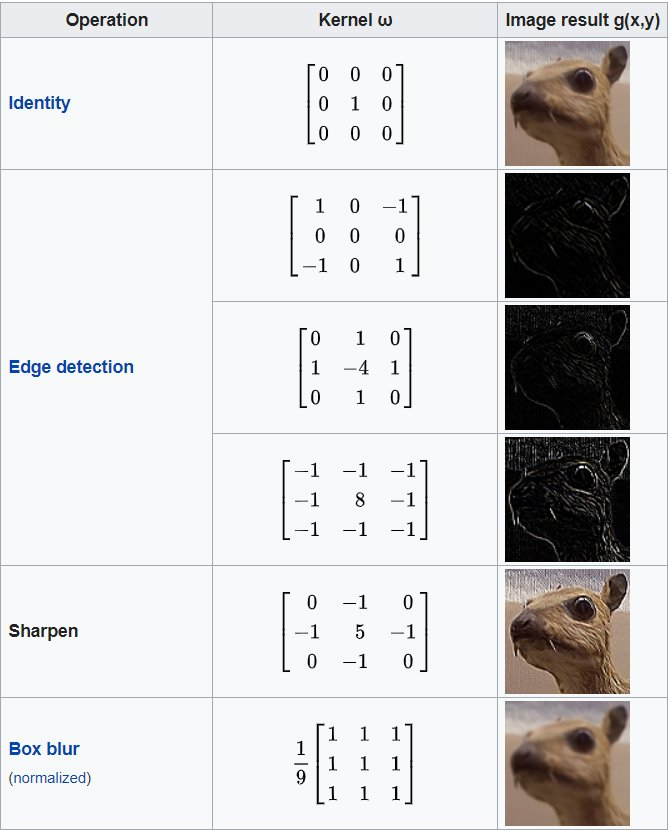
\includegraphics[width=0.6\textwidth]{images/1/image.png}
        \caption{}
\end{figure}
%
%
%
%
%
%
%
%
%
\subsection{Convolutional neutral network}
Mạng CNN là một tập hợp của các lớp Convolution được xếp chồng lên nhau. CNN sử dụng các hàm kích hoạt phi tuyến (như ReLU và tanh) để tạo ra thông tin trừu tượng. Sau khi đi qua các lớp này, mạng thu được trọng số trong các node và tạo ra thông tin trừu tượng cho các lớp kế tiếp.

\noindent Đặc điểm quan trọng của mô hình CNN là tính bất biến và tính kết hợp. Điều này có ảnh hưởng đến độ chính xác của mô hình khi đối tượng được chiếu từ nhiều góc độ khác nhau. \textbf{Pooling layer được sử dụng để tạo tính bất biến đối với các biến đổi như dịch chuyển, co giãn và quay}.

\noindent Các layer convolution giúp thể hiện các cấp độ biểu diễn từ mức độ thấp đến cao, kết hợp thông tin từ các filter. Liên kết giữa các layer đảm bảo kết nối cục bộ hiệu quả nhất. Mỗi nơ-ron trong lớp tiếp theo được tạo ra từ kết quả của convolution thuộc layer trước đó.

\noindent\textbf{ Pooling/subsampling layer được sử dụng để chọn lọc thông tin quan trọng và loại bỏ nhiễu}.
\begin{figure}[htbp]
        \centering
        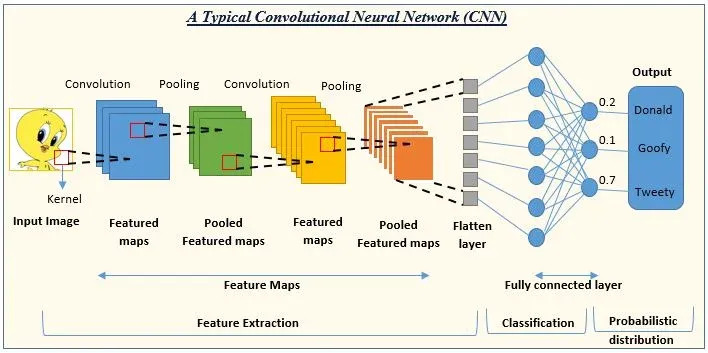
\includegraphics[width=0.6\textwidth]{images/2a-sign/cnn.jpg}
        \newline
        \caption{Cấu trúc của mạng CNN}
\end{figure}
\textbf{Cấu trúc cơ bản nhất của 1 CNN gồm 3 phần là:}
\begin{itemize}
    \item \textbf{Local receptive field (trường cục bộ):}Nhiệm vụ của trường cục bộ là phân tách và lọc dữ liệu cũng như thông tin ảnh, sau đó chọn ra các vùng ảnh có giá trị sử dụng cao nhất. 
    \item \textbf{Shared weights and bias (trọng số chia sẻ):}Trong mạng CNN, thành phần này có tác dụng giảm thiểu tối đa lượng tham số có tác dụng lớn. Trong mỗi convolution sẽ chứa nhiều feature map khác nhau, mỗi feature lại có khả năng giúp nhận diện một số feature trong ảnh. 
    \item \textbf{Pooling layer (lớp tổng hợp):}Pooling layer là lớp cuối cùng, với khả năng đơn giản hóa thông tin đầu ra. Khi đã hoàn tất tính toán và quét qua các lớp, pooling layer sẽ được tạo ra nhằm mục đích lược bớt các thông tin không cần thiết và tối ưu đầu ra. Điều này giúp người dùng nhận được kết quả ưng ý và đúng với yêu cầu hay mong muốn.
\end{itemize}
\begin{figure}[htbp]
        \centering
        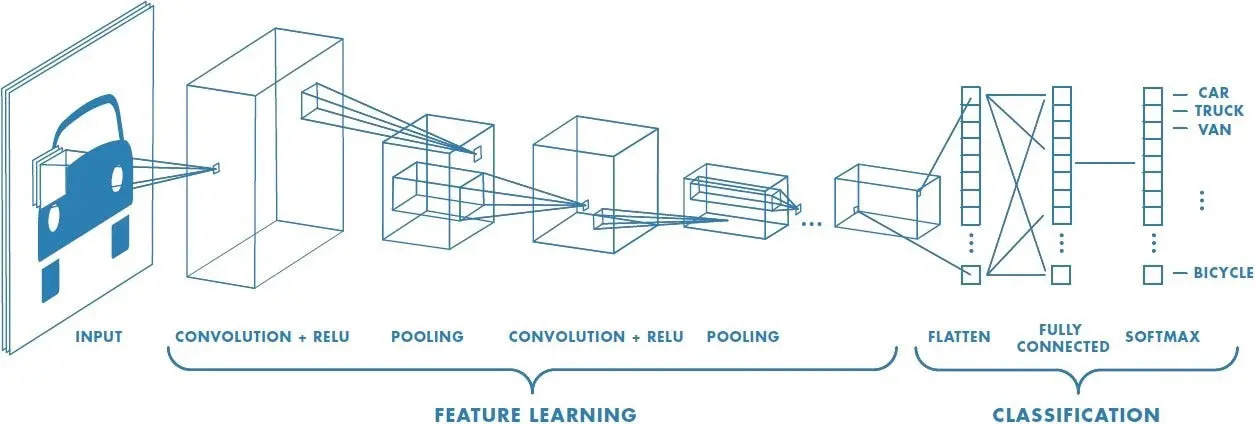
\includegraphics[width=0.7\textwidth]{images/2a-sign/cnn1.jpg}
        
\end{figure}

